\documentclass[../../tc_tp6_main.tex]{subfiles}

\begin{document}

%capítulo
\chapter{Dise\~no de VCO}

En esta secci\'on, se propondr\'a una implementaci\'on de un oscilador controlado por tensi\'on, mejor conocido como VCO (por sus siglas en ingl\'es: \textit{voltage-controlled oscillator}). El mismo recibir\'a como entrada una tensi\'on constante de entre 0V y 5V, y producir\'a a la salida una se\~nal senoidal de 1V de amplitud, cuya frecuencia variar\'a linealmente seg\'un la tensi\'on de entrada entre 1kHz y 10kHz. 


\section{Introducci\'on: el VCO}

El VCO es un oscilador electr\'onica cuya frecuencia de salida depende de la tensi\'on de entrada recibida. Entre sus aplicaciones se destacan su uso en los PLLs, as\'i como la generaci\'on de funciones en s\'i misma.\par

Seg\'un la forma de la se\~nal de salida, los VCOs (as\'i como los osciladores en general) pueden categorizarse como:

\begin{itemize}
	\item \underline{arm\'onicos}: la salida es una se\~nal senoidal. Se implementan generalmente con circuitos LC con compensaci\'on de las p\'erdidas  u osciladores de cristal.
	\item \underline{de relajaci\'on}: la salida es una se\~nal triangular o una rampa.
\end{itemize}

En ambos casos, el par\'ametro fundamental de un VCO es su sensibilidad $k$, que es aquella que establece la relaci\'on entre la tensi\'on de la entrada y la frecuencia fundamental de la salida:

\begin{equation}
	f_{OUT} = k V_{IN}
\end{equation}

Otras caracter\'isticas que pueden resultar de inter\'es en un VCO refieren, en cambio, a la calidad de la salida:

\begin{itemize}
	\item \underline{jitter}: indica qu\'e tan estable se mantiene la frecuencia cuando la tensi\'on de entrada se mantiene constante (salvo quiz\'as por el ruido que pueda tener montado la continua de entrada).
	\item \underline{THD (total harmonic distortion)}: indica qu\'e porcentaje de la potencia de la frecuencia fundamental de la salida se encuentra en sus arm\'onicos. Desde ya, este par\'ametro es relevante s\'olo en el caso de que el VCO sea arm\'onico.
\end{itemize}

\newpage

\section{Dise\~no}


\subsection{Oscilador}
En este caso en particular, el VCO que se implementar\'a es el siguiente:


\begin{figure}[H]
	\centering
	\begin{circuitikz}
		\draw
		(5,7) node[op amp, yscale=-1] (oa) {}		
		(10,6.5) node[op amp] (comp) {}			
		(3,1.5) node[npn, xscale=-1](npn){}		
		
		(0,7.5) node[left] {$V_{IN}$}
		(0,7.5) to [short, o-*] (1,7.5) 
		to [R = 10k$\Omega$, -*] (3, 7.5) %node[below]{$\nicefrac{V_{IN}}{2}$}
		to [short] (oa.+)	
		(3, 7.5) to [R, l_=10k$\Omega$] (3, 9.5) node[ground, yscale=-1]{}	
		
		(1, 7.5) to [short] (1, 6.5)
		to [R, l_=$2R$, -*] (3, 6.5) node[above]{$\nicefrac{V_{IN}}{2}$}
		to [short] (oa.-)
		(3, 6.5) to [short, -*, , i^>=$\nicefrac{V_{IN}}{4R}$] (3, 5.5)
		to [R = $R$] (npn.C)
		
		(comp.-) to [short, -*] (oa.out)
		to [short] (oa.out) -- ++ (0, -1.5)
		to [C=$C$] (3, 5.5)
		
		(oa.out) to [short, -o] (6.2, 7.5) node[above]{$V_{TR}$}	
		
		(comp.+) to [short] (8, 6)
		to [short, -*] (8,5)
		to [R, l_=1k$\Omega$] (8,3) node[ground]{}
		
		(8,5) to [vR, l_=5k$\Omega$, -*] (11.5,5)
		to [short, -*] (11.5, 6.5) to [short] (comp.out)
		(11.5, 6.5) to [short, -o] (12, 6.5) node[right]{$V_{SQ}$}
		
		(11.5, 5) to [short] (11.5, 1.5)
		to [R=1k$\Omega$] (npn.B)
		
		(npn.E) node[ground]{}		
	;\end{circuitikz}
	
	\caption{\textit{Voltage-controlled oscillator} con salidas triangular y cuadrada}
	\label{fig:vco}
\end{figure}

En la entrada no inversora del primer operacional, un divisor resistivo fija una tensi\'on de $\nicefrac{V_{IN}}{2}$, que se ver\'a replicada en el terminal inversor (considerando el operacional como ideal), y por lo tanto entre este terminal y la entrada la corriente ser\'a siempre de $\nicefrac{V_{IN}}{4R}$. Dependiendo de qu\'e ocurra con el transistor, que se est\'a utilizando como \textit{switch}, las consecuencias de esto ser\'an:

\begin{itemize}
	\item si el transistor conduce, por la resistencia $R$ circula $\nicefrac{V_{IN}}{2R}$, y por lo tanto por el capacitor debe aportar $\nicefrac{V_{IN}}{4R}$ desde la salida del operacional a la entrada inversora (nuevamente considerando ideal al \textit{opamp}).
	\item si el transistor no conduce, toda la corriente que llega al terminal no inversor deber\'a seguir por el capacitor, y por lo tanto su valor tambi\'en ser\'a $\nicefrac{V_{IN}}{4R}$, pero en el sentido contrario que en el caso anterior.
\end{itemize}

Utilizando la ecuaci\'on fundamental del capacitor $i_C = C \frac{dV_C}{dt}$, se obtiene que:
\begin{equation}
	\Delta V_C = \pm \frac{V_{IN}}{4RC}\cdot\Delta t
	\label{eq:vc}
\end{equation}

Por lo tanto, la salida del primer operacional es una rampa definida por la ecuaci\'on:

\begin{equation}
	V_{TR} = \frac{V_{IN}}{2} + V_C = \frac{V_{IN}}{2} \cdot (1 \pm \frac{\Delta t}{2RC})
	\label{eq:vtr}	
\end{equation}

Queda entonces definir qu\'e es lo que sucede con la tensi\'on en la base del transistor, puesto que ser\'a esta la que determine si la pendiente de la rampa es positiva o negativa. \par

Esta tensi\'on est\'a controlada por el segundo \textit{opamp}. Por la retroalimentaci\'on positiva identificamos que no cumple otra funci\'on sino la de Schmidt trigger. Como $V_{out} = A_{vol} \cdot (V^+ - V^-)$, pero esta tensi\'on est\'a a su vez limitada por la saturaci\'on del operacional, $V_{SQ}$ tiene s\'olo dos estados estables:

\begin{itemize}
	\item si $V^+ > V_{TR}$, entonces $V_{SQ} = V_{SAT}$, lo cual a su vez fija $V^+$ en una fracci\'on de $V_{SAT}$, cuyo valor depender\'a de la resistencia variable y llamaremos $V_{TH}$ (tensi\'on de trigger high).
	\item si $V^+ < V_{TR}$, entonces $V_{SQ} = -V_{SAT}$. Lo que ocurre con $V^+$ es an\'alogo al caso anterior, de donde se obtiene $V_{TL}$ (tensi\'on de trigger low).
\end{itemize}

Por lo tanto, la rampa descripta por la ecuaci\'on \ref{eq:vtr} cambiar\'a de pendiente positiva a negativa cuando $V_{TR} = V_{TH}$, y viceversa cuando $V_{TR} = V_{TL}$. Reemplazando entonces $\Delta V$ por $V_{TH} - V_{TL}$ y $\Delta t$ por $\frac{1}{2f_0}$, obtenemos que:

\begin{equation}
	f_0 = \frac{V_{IN}}{8\cdot RC\cdot (V_{TH} - V_{TL})}
	\label{eq:frecuencia}
\end{equation}

Si bien hemos cumplido hasta aqu\'i con dise\~nar un VCO, hay una serie de problemas con esta implementaci\'on en cuanto a lo pedido por la consigna, las cuales se enfrentar\'an de la siguiente manera:

\begin{itemize}
	\item Las tensiones de trigger dependen fuertemente de las tensiones de saturaci\'on del \textit{opamp}. Si bien sabemos que si $V_{CC} = 15\mathrm{V}$, $V_{SAT}$ estar\'a alrededor de los 12V, no podemos saber a priori con cu\'anta tensi\'on exacta saturar\'a cada integrado. Incluso si se midiese antes de armar el circuito, si se quemase el integrado habr\'ia que volver a medir y cambiar una de las resistencias del divisor de tensi\'on. Por esta raz\'on se utiliza un preset en esta etapa.
	\item Con esta configuraci\'on, cuando la tensi\'on de entrada es 0V la salida tambi\'en lo es. Esto se contradice con nuestro objetivo de tener siempre salidas de entre 1kHz y 10kHz. Por lo tanto, se efectuar\'a una transformaci\'on lineal tal que cuando $V_{IN} = 0\mathrm{V}$, al VCO se entre con 1V. Como queremos adem\'as que la frecuencia m\'axima sea 10kHz, esto implica que cuando $V_{IN}=5\mathrm{V}$, se deben tener 10V a la entrada del VCO.
	\item Este es un oscilador de relajaci\'on, y no uno arm\'onico como necesitamos. Se necesita, pues, efectuar una conversi\'on de triangular a senoidal. 
\end{itemize}

Dadas estas consideraciones, se eligieron los valores de los componentes:

\begin{equation}
	\left\{
	\begin{aligned}
		C &= 10\mathrm{nF} \\
		R &= 1.25\mathrm{k}\Omega
	\end{aligned}
	\right.
\end{equation}

De esta manera, se puede usar un capacitor multicapa y tener una tolerancia del 5\% con la cual las otras tecnolog\'ias disponibles no cuentan, y los valores de las resistencias $R$ y $2R$ se aproximaron con una \'unica combinaci\'on serie para cada caso.\par

En cuanto a los operacionales, se utiliz\'o el integrado TL074. De esta manera, se cubrieron los 4 \textit{opamps} que requerir\'a la totalidad del circuito (como se ver\'a a la brevedad). Se prioriz\'o en la elecci\'on cumplir las recomendaciones del libro \textit{Design with Operational Amplifiers and Analog Integrated Circuits} de Sergio Franco, a saber: un operacional FET con baja corriente de \textit{bias} (65pA) \footnote{Informaci\'on obtenida de la \href{http://www.ti.com/lit/ds/symlink/tl074.pdf}{\underline{\textit{data sheet}}} del operacional (consultado: 08/11/18).} y buen \textit{slew rate} (13$\nicefrac{\mathrm{V}}{\mu\mathrm{s}}$). A su vez, este operacional presenta buenas caracter\'isticas en cuanto al ruido (mejores que las del TL084, por ejemplo), como un 0.003\% de THD, lo cual es fundamental en este circuito si queremos obtener una baja distorsi\'on de la se\~nal final.\par 

Por \'ultimo, el transistor utilizado fue un 2N2222, puesto que est\'a dise\~nado espec\'ificamente para utilizarlo como \textit{switch}. Para limitar la corriente de base del mismo se agreg\'o una resistencia de 1k$\Omega$ entre la misma y el \textit{output} del Schmidt trigger, tal como se ilustra en la figura \ref{fig:vco}. \par

En cuanto a consideraciones adicionales que se tuvieron para mejorar la se\~nal de entrada, se agregaron capacitores de desacople de 100nF entre $V_{CC}$ y $V_{EE}$ y \textit{ground}. Los mismos se colocaron lo m\'as cerca posible del integrado, a fin de contrarrestar los efectos de la inductancia de las pistas de cobre. El prop\'osito de estos capacitores es estabilizar la tensi\'on de alimentaci\'on, lo cual es cr\'itico en este circuito, puesto que la frecuencia depende fuertemente de la misma a trav\'es de la tensi\'on de saturaci\'on. De esta manera, se busc\'o reducir el \textit{jitter} de la salida.\par

Por \'ultimo, cabe destacar que la impedancia de salida de este circuito es s\'olo la salida de un operacional. Esto es \'util puesto que se debe agregar una etapa de conversi\'on de triangular a senoidal, y dada esta caracter\'istica se puede considerar que las etapas no se cargar\'an entre s\'i. 

\newpage

\subsection{Transformaci\'on lineal [0V; 5V] a [1V; 10V]}

Se quiere obtener un circuito que efect\'ue la transformaci\'on lineal:
\begin{equation}
	V_{OUT} = \frac{9}{5} \cdot V_{IN} + 1\mathrm{V} 
	\label{eq:tl}
\end{equation}

Se utiliz\'o entonces un circuito sumador inversor, utlizando $V_{CC} = 15\mathrm{V}$ para generar el \textit{offset}. El mismo se encuentra ilustrado en la figura \ref{fig:sumador}.
\begin{figure}[H]
	\centering
	\begin{circuitikz}
		\draw
		(4,3) node[op amp, yscale=-1](oa){}		
		
		(0,5) node[left]{+15V} 
		to [R, l^=$R_1$, o-] (2.8,5)
		to [short] (oa.+)
		
		(0,3.5) node[left]{$V_{IN}$}
		to [R, l^=$R_2$, o-*] (oa.+)
		
		(oa.-) to [short, -*] (2.8,1.5)
		to [R=$R_4$] (2.8, -0.5) node[ground]{}
		
		(2.8, 1.5) to [R=$R_3$] (5.2, 1.5)
		to [short, -*] (oa.out) 
		to [short, -o] (5.7, 3) node[right] {$V_{OUT}$} 
	;\end{circuitikz}
	\caption{Sumador no inversor}
	\label{fig:sumador}
\end{figure}
 Por superposici\'on se puede obtener que la salida de este circuito es:

\begin{equation}
	V_{OUT} = \left( \frac{1 + \frac{R_3}{R_4}}{R_1 + R_2} \right) \cdot \left( R_1 \cdot V_{IN} + R_2 \cdot 15\mathrm{V}\right)
\end{equation}

Combinando este resultado con el obtenido en \ref{eq:tl}, se obtiene que las relaciones entre los componentes son:

\begin{equation}
	1 + \frac{R_3}{R_4} = \frac{1}{15} \cdot \left( 1 + \frac{R_1}{R_2} \right) = \frac{9}{15} \cdot \left( 1 + \frac{R_2}{R_1} \right)
\end{equation}

Se utilizaron entonces los siguientes valores, utilizando una combinaci\'on serie para $R_2$ y $R_3$:

\begin{equation}
	\left\{ \begin{aligned}
	R_1 &= 33\mathrm{k}\Omega   	&  R_2 &= 1.22\mathrm{k}\Omega   \\
	R_3 &= 13\mathrm{k}\Omega 	&  R_4 &= 15\mathrm{k}\Omega
	 \end{aligned}  \right.
\end{equation}

Se observa, adem\'as, que la impedancia de salida de este circuito es solamente la del operacional. Por lo tanto, como la impedancia de entrada del VCO es en cambio una combinaci\'on de resistencias en el orden de los kiloohm, podemos considerar que estas etapas no se cargan entre s\'i.

\newpage 

\subsection{Conversor triangular a senoidal}

Si bien una se\~nal triangular puede convertirse en una senoidal mediante un filtro apropiado, en este caso es de inter\'es que este proceso sea independiente de la frecuencia. Por lo tanto, se utiliz\'o el circuito de la figura \ref{fig:pardif}.

\begin{figure}[H]
	\centering
	\begin{circuitikz}
		\draw
		(5,5) node[npn](n1){}		
		(8,5) node[npn, xscale=-1](n2){}		

		(1.5, 5) node[left]{$V_{TR}$}
		to [vR=100k$\Omega$, o-*] (4, 5) 
		to [R, l_=2.2k$\Omega$] (4, 3) node[ground]{}
		(4,5) to [short] (n1.B)		
		
		(n1.E) to [short, -*] (5, 3.5)
		to [R=390R, -*] (8,3.5)
		to (n2.E)
		
		(5, 3.5) to [short] (5, 1.5)
		to [R=100k$\Omega$] (8,1.5)
		to [short] (8, 3.5)
		
		(6.5, -1) node[below]{$V_{EE}$}
		to [R=18k$\Omega$, o-] (6.5, 1.3) node[inputarrow, rotate=90]{}
		
 		(n2.B) to [short, -*] (9,5)
 		to [R=2.2k$\Omega$] (9,3) node[ground]{}
 		
 		(n1.C) to [R=10k$\Omega$] (5,8.5)
 		to [short] (8,8.5)
 		to [R=10k$\Omega$] (n2.C)
 		
 		(6.5,8.5) to [short, *-o] (6.5, 9) node[above]{$V_{CC}$}
 		
 		(11,6) node [op amp, scale=0.5](oa) {}
 		(oa.-) to [short, -*] (5, 6.25) 		
 		(oa.+) to [short] (10, 5.75) node[ground]{}
 		
		(oa.-) to [short] (10, 6.25)
		to [short, *-] (10, 7)
		to [vR=5k$\Omega$] (12,7)
		to [short, -*] (12, 6) 
		to [short, -o] (12.5,6) node [right]{$V_{SIN}$} 		
 		(oa.out) to [short] (12,6)
 		
	;\end{circuitikz}
	
	\caption{Conversor de onda triangular a senoidal}
	\label{fig:pardif}
\end{figure}

Este circuito consiste en un par diferencial, cuya salida est\'a controlada en ganancia por el preset del operacional. El prop\'osito del par diferencial es obtener una transferencia cuyas caracter\'isticas permitan aproximar una senoidal, lo cual se logra explotando las caracter\'siticas no lineales de los transistores, como se ilustra en la figura \ref{fig:curvatransistor}.\par

Sin embargo, esto requiere entrar con exactamente con una triangular de amplitud tal que sea lo suficientemente grande como para superar la zona lineal cercana al origen, pero no lo suficiente como para saturar a los transistores. Si bien sabemos que esto ocurrir\'a con aproximadamente 400mV pico a pico, esto depender\'a fuertemente de los transistores utilizados, y es fundamental que este ajuste sea preciso. A su vez, la tensi\'on de entrada depender\'a de la calibraci\'on que previamente se haya realizado en el VCO. Por esta raz\'on se incluy\'o el preset del divisor resistivo en la entrada. \par

A su vez, este par diferencial funcionar\'a apropiadamente si ambos transistores est\'an trabajando con la misma corriente de colector en todo momento. Esto es imposible de obtener de manera exacta en dos transistores distintos, y por eso se incluy\'o el segundo preset entre los emisores. \par

En este caso, los transistores utilizados fueron dos BC548, puesto que los mismos son espec\'ificos para amplificaci\'on (al contrario del caso anterior).\par 

\begin{figure}[H]
	\centering
	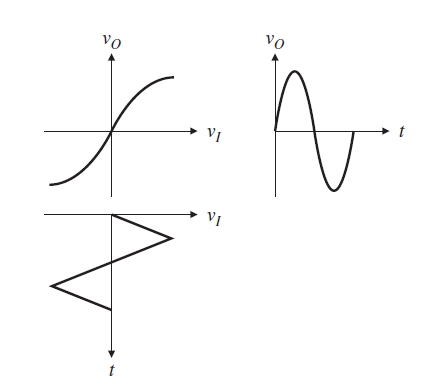
\includegraphics[scale=0.8]{imagenes/triang-sin.png}
	\caption{Conversi\'on de triangular a senoidal utilizando las zonas no lineales del transistor}
	\label{fig:curvatransistor}
\end{figure}


\subsection{Calibraci\'on}

En su totalidad, este circuito cuenta con cuatro resistencias variables. Para obtener una salida que cumpla las caracter\'isticas pedidas, los mismos deben ajustarse en el siguiente orden:

\begin{enumerate}
	\item Con el preset del VCO se ajusta la \underline{frecuencia} de salida correspondiente a cada tensi\'on de entrada. Por ejemplo, puede conectarse la entrada a \textit{ground} (es decir setear $V_{IN}$ en 0V) y ajustar el preset hasta obtener en la salida una se\~nal de frecuencia 1kHz. Para esto puede observarse tanto la salida final del circuito como las salidas triangular o cuadrada del VCO.
	\item Se ajusta el preset que se encuentra entre los emisores de los BC548 para lograr \underline{simetr\'ia} en la salida.
	\item Se ajusta el preset de la entrada del conversor triangular a senoidal hasta obtener una \underline{forma senoidal} en la salida.
	\item Se lleva la \underline{ganancia} del sistema con el preset de la salida, hasta llevar la tensi\'on final a 1V de amplitud. 
\end{enumerate}

\newpage

\section{Resultados}

Se verific\'o etapa por etapa el correcto funcionamiento del circuito.

\subsection{Transformaci\'on lineal}

Realizando un DC \textit{sweep} y utilizando el modo XY del oscilopio, se midieron las salidas correspondientes para las tensiones del rango especificado por la consigna.

\begin{figure}[H]
	\centering
	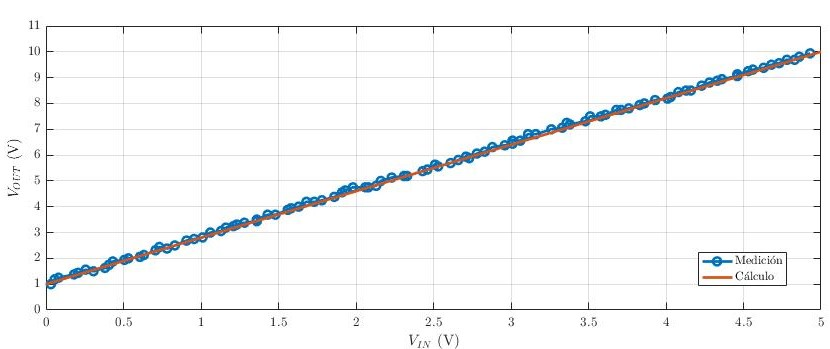
\includegraphics[scale=0.71]{imagenes/tc_tp6_ej3_tl.jpg}
	\caption{Transferencia de la transformaci\'on lineal}
\end{figure}

Si bien el \textit{offset} se logr\'o obtener de manera precisa, no as\'i la pendiente: no se logra llegar a los 10V te\'oricos con 5V en la entrada. Por lo tanto, se espera que al calibrar el VCO para que la frecuencia correspondiente a 0V sea 1kHz, no se llegue a los 10kHz con 5V, sino con una tensi\'on levemente superior.

\subsection{Oscilador}
\begin{figure}[H]
	\centering
	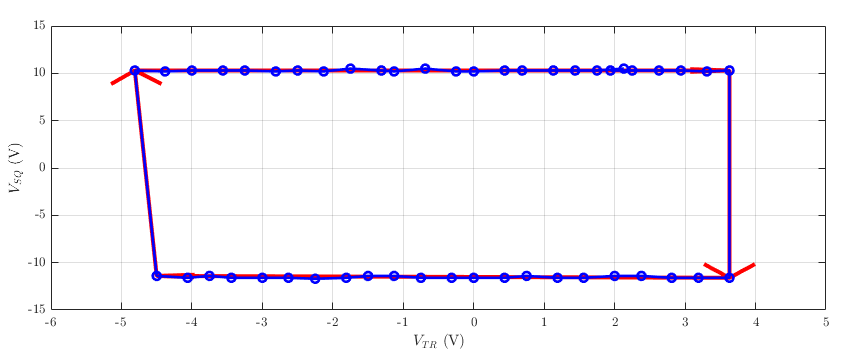
\includegraphics[scale=0.71]{imagenes/tc_tp6_ej3_st.png}
	\caption{Transferencia del Schmidt trigger}
\end{figure}


\subsection{Conversi\'on triangular a senoidal}

\begin{table}[H]
	\centering
	\begin{tabular}{|c|c|}
	\hline
	\begin{tabular}[c]{@{}c@{}}Frecuencia\\   fundamental (kHz)\end{tabular} 	& THD (\%)	\\ \hline \hline
	1.11                                                                     					& 0.846    		\\ \hline
	2.92                                                                     					& 0.405    		\\ \hline
	4.98                                                                    					& 0.252    		\\ \hline
	6.21                                                                     					& 0.307   		\\ \hline
	7.68                                                                    					& 1.023    		\\ \hline
	10.0                                                                     					& 1.478    		\\ \hline
	\end{tabular}
	\caption{Distorsi\'on arm\'onica de la salida a distintas frecuencias}
\end{table}


\begin{table}[H]
	\centering
	\begin{tabular}{|c||c|c|c|c|}
	\hline
	$V_{IN}$ (V) 	& Frecuencia media (kHz) 	& M\'inima (kHz) 	& M\'axima (kHz) 	& Desviaci\'on est\'andar (kHz) 	\\ \hline \hline
	0.0          		& 1.12                   		& 1.12                      	& 1.13                      	& $2.10\times 10^{-03}$           	\\ \hline
	1.1          		& 3.22                   		& 3.21                      	& 3.23                      	& $6.60\times 10^{-03}$           	\\ \hline
	2.0          		& 4.88                   		& 4.85                      	& 4.90                      	& $4.70\times 10^{-03}$           	\\ \hline
	3.1          		& 6.76                   		& 6.71                     	& 6.80                      	& $1.50\times 10^{-02}$           	\\ \hline
	4.1          		& 8.49                   		& 8.40                      	& 8.60                      	& $2.40\times 10^{-02}$          	\\ \hline
	5.0          		& 10.1                   		& 10.0                      	& 10.2                      	& $4.40\times 10^{-02}$           	\\ \hline
	\end{tabular}
	\caption{\textit{Jitter} de la salida para distintas tensiones de entrada}
\end{table}




\section{Conclusiones}

DIO TODO IMPECABLE VIEJA NI NO VIMO

\end{document}
